% !TeX root = tesis.tex

En esta sección introducimos las curvas elípticas sobre un cuerpo, y las dotamos de una estructura de grupo abeliano. Las curvas elípticas presentan propiedades de seguridad criptográfica favorables, en particular, para niveles de seguridad comparables, los grupos de curvas elípticas permiten tamaños de parámetros significativamente menores que los grupos multiplicativos clásicos.

\begin{definition}[Curva elíptica]
	Sea $\K$ un cuerpo con $\charac{\K} \neq 2,3$. Una curva elíptica $\E$ sobre $\K$ es una curva, junto con un punto distinguido $\OO$, que puede describirse mediante una ecuación de la forma
	$$\E: y^2 = x^3 + ax + b, \quad a,b \in \K,$$
	y sujeta a la condición de no singularidad $4a^3 + 27b^2 \neq 0$.
	
	El conjunto de puntos de la curva elíptica sobre $\K$ se define como
	$$\E(\K) = \{(x,y) \in \K \times \K: y^2 = x^3 + ax + b\} \cup \{\OO\},$$
	donde $\OO$ denota el punto del infinito o punto identidad.
\end{definition}

La condición de no singularidad garantiza que la curva no posee puntos singulares, y por lo tanto que la curva es lisa. Es decir, si consideramos la función en dos variables $F(x,y) = y^2 - x^3 - ax - b$, sus derivadas parciales son $\frac{\partial F}{\partial x}(x,y) = -3x^2 - a$, y $\frac{\partial F}{\partial y}(x,y) = 2y$. Un punto de la curva es singular si ambas derivadas parciales de $F$ se anulan en él.

\begin{definition}[Definición geométrica de suma en curvas elípticas]
	Sea $\K$ un cuerpo, y $\E(\K)$ una curva elíptica. Dados $P, Q \in \E(\K)$, se define la suma $+: \E(\K) \times \E(\K) \to \E(\K)$ desde una perspectiva geométrica, como:
	\begin{enumerate}
		\item Se considera la recta que pasa por $P$ y $Q$. En el caso particular $P = Q$, se toma la recta tangente a la curva en $P$. En el caso particular $Q = -P$, la recta es vertical.
		\item La recta interseca a la curva elíptica en un tercer punto $R$ (contando multiplicidades).
		\item Si $R'$ es la reflexión de $R$ por el eje $x$, se define $P + Q := R'$. En el caso particular de la recta vertical, tenemos $Q = -P$ y se define $P + Q := \OO$.
	\end{enumerate}
\end{definition}

\begin{figure}[!t]
	\centering
	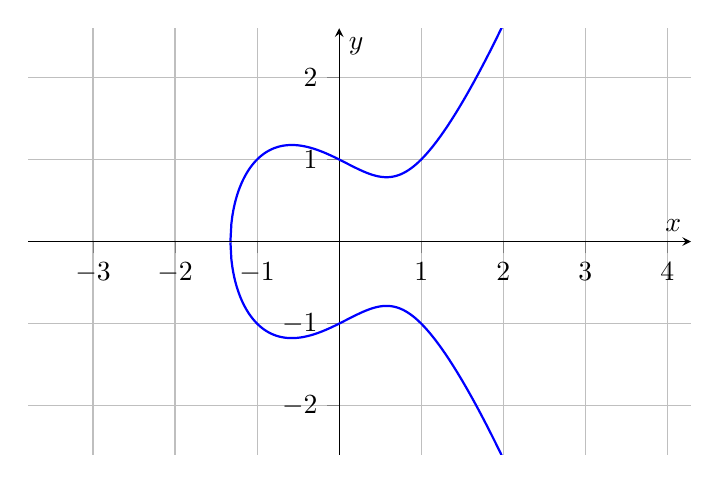
\begin{tikzpicture}
		\begin{axis}[
			axis lines = middle,
			axis equal,
			xlabel = $x$,
			ylabel = $y$,
			xmin = -1.6,
			xmax = 2.1,
			ymin = -2.6,
			ymax = 2.6,
			samples = 300,
			domain = -1.3247:2,
			width = 10cm,
			height = 7cm,
			grid = both,
			tick align = outside
			]
			
			% Rama superior
			\addplot[blue, thick] {sqrt(x^3 - x + 1)};
			
			% Rama inferior
			\addplot[blue, thick] {-sqrt(x^3 - x + 1)};
		\end{axis}
	\end{tikzpicture}
	\caption{Curva elíptica real $\E(\mathbb{R})$ dada por $y^2=x^3-x+1$. La figura muestra las dos ramas $y=\pm\sqrt{x^3-x+1}$ en el plano real; la condición de no singularidad garantiza que esta curva pueda equiparse con la operación geométrica de suma de puntos junto con el punto en el infinito $\OO$.}
	\label{fig:curva-eliptica-real}
\end{figure}


La introducción del punto $\OO$ es necesaria para que la suma de puntos esté definida en todos los casos, en particular cuando se suman puntos opuestos cuya recta secante es vertical. Sin este punto adicional, la operación no sería cerrada en $\E(\K)$. Esta operación cumple el resto de propiedades para poder considerar a $(\E(\K), +)$ como un grupo abeliano:
\begin{itemize}
	\item $P + \OO = \OO + P = P$ para todo $P \in \E(\K)$ (elemento neutro).
	\item $P + (-P) = \OO$ para todo $P \in \E(\K)$ (elemento inverso). Un detalle geométrico relevante es que $-P$ se obtiene al reflejar $P$ por el eje $x$.
	\item $P + (Q + R) = (P + Q) + R$ para todos $P, Q, R \in \E(\K)$ (asociatividad).
	\item $P + Q = Q + P$ para todos $P, Q \in \E(\K)$ (conmutatividad).
\end{itemize}

Por convención, utilizaremos notación aditiva en vez de multiplicativa al trabajar con grupos de curva elíptica. Dados $n \in \N$ y $P \in \E(\K)$, podemos definir $nP := P + P + \ldots + P$, donde hay $n$ sumandos.

Al pasar a considerar curvas elípticas sobre cuerpos finitos, es decir curvas de la forma $\E(\Fq)$ con $q = p^k$, $p$ primo y $\charac{\Fq} \neq 2,3$, la interpretación geométrica deja de ser literal, aunque sigue siendo una guía conceptual valiosa. La estructura de grupo abeliano se preserva, y en particular la operación de suma continúa estando bien definida. Sin embargo, en este contexto ya no resulta conveniente describir la suma en términos geométricos, sino mediante fórmulas algebraicas explícitas.

\begin{definition}[Definición algebraica de suma en curvas elípticas]
	Sea $\K$ un cuerpo finito, sea $\E(\K)$ una curva elíptica y sean $P, Q \in \E(\K)$. Se define la suma $+: \E(\K) \times \E(\K) \to \E(\K)$ desde una perspectiva algebraica mediante fórmulas explícitas y el siguiente algoritmo:
	\begin{enumerate}
		\item Si $P = \OO$, entonces $P + Q := Q$. Similarmente, si $Q = \OO$, entonces $P + Q := P$.
		\item Si $P, Q \neq \OO$, entonces son puntos de la forma $P = (x_P, y_P)$, $Q = (x_Q, y_Q)$ con coordenadas en $\Fq$. Si $Q = -P$, lo que es equivalente a $x_P = x_Q$ y $y_P = -y_Q$, entonces $P + Q := \OO$.
		\item Se calcula la pendiente $\lambda$ de la recta que pasa por $P$ y $Q$.
		\begin{itemize}
			\item En el caso $P = Q$, es una recta tangente a $P$ y $\lambda := \frac{3x_P^2 + a}{2y_P}$.
			\item En el caso $P \neq Q$, se calcula de forma usual: $\lambda := \frac{y_Q - y_P}{x_Q - x_P}$.
		\end{itemize}
		\item Para $x^* := \lambda^2 - x_P - x_Q$ y $y^* = \lambda(x_P - x^*) - y_P$, se define $P + Q := (x^*, y^*)$.
	\end{enumerate}
\end{definition}

Podemos ver un ejemplo concreto sobre la curva $\E(\F_{19})$ dada por la ecuación $y^2 = x^3 - x + 1$. Tomemos
$P = (2,8), Q = (3,5) \in \E(\F_{19})$. Como $P \neq Q$ y $Q \neq -P$, hacemos los siguientes cálculos:
$$\begin{aligned}
	\lambda = \frac{y_Q - y_P}{x_Q - x_P} = \frac{5 - 8}{3 - 2} = -3 \equiv 16 \pmod{19}, \\
	x^* = \lambda^2 - x_P - x_Q = 16^2 - 2 - 3 = 251 \equiv 4 \pmod{19}, \\
	y^* = \lambda(x_P - x^*) - y_P = 16(2 - 4) - 8 = -40 \equiv 17 \pmod{19}.
\end{aligned}$$
Por lo tanto, $P + Q = (4,17)$.

\begin{figure}[!t]
	\centering
	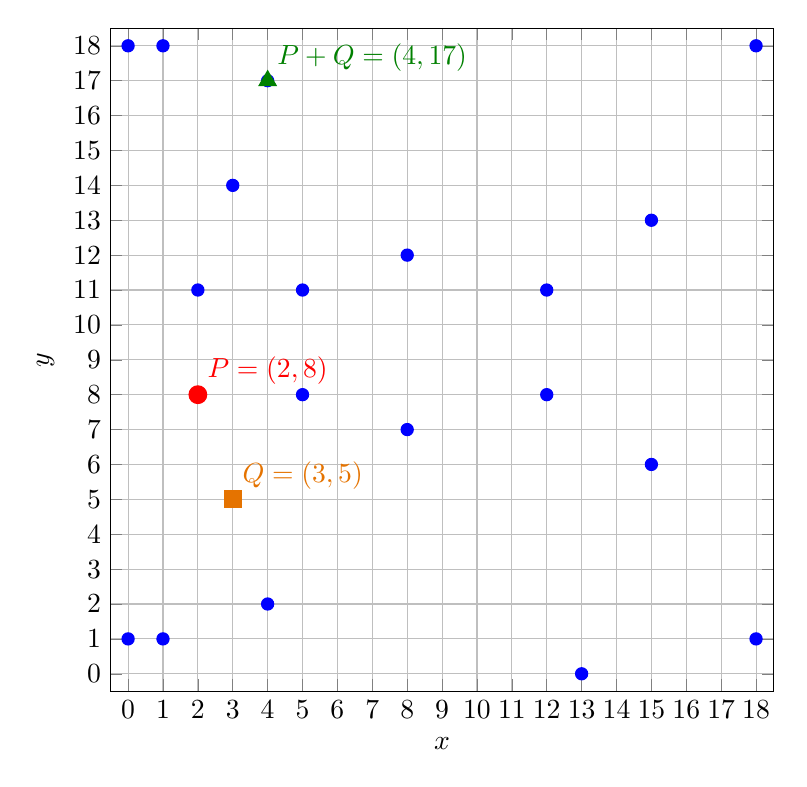
\begin{tikzpicture}
		\begin{axis}[
			axis equal,
			xmin = -0.5,
			xmax = 18.5,
			ymin = -0.5,
			ymax = 18.5,
			xtick = {0,...,18},
			ytick = {0,...,18},
			grid = both,
			xlabel = $x$,
			ylabel = $y$,
			width = 10cm,
			height = 10cm
			]
			\addplot[
				only marks,
				mark = *,
				mark size = 2.2pt,
				blue
			]
			coordinates {
				(0,1) (0,18)
				(1,1) (1,18)
				(2,8) (2,11)
				(3,5) (3,14)
				(4,2) (4,17)
				(5,8) (5,11)
				(8,7) (8,12)
				(12,8) (12,11)
				(13,0)
				(15,6) (15,13)
				(18,1) (18,18)
			};

			\addplot[
				only marks,
				mark = *,
				mark size = 3.2pt,
				red
			]
			coordinates {(2,8)};
			\addplot[
				only marks,
				mark = square*,
				mark size = 3.0pt,
				orange!90!black
			]
			coordinates {(3,5)};
			\addplot[
				only marks,
				mark = triangle*,
				mark size = 3.6pt,
				green!50!black
			]
			coordinates {(4,17)};

			\node[anchor=south west, text=red] at (axis cs:2,8) {$P=(2,8)$};
			\node[anchor=south west, text=orange!90!black] at (axis cs:3,5) {$Q=(3,5)$};
			\node[anchor=south west, text=green!50!black] at (axis cs:4,17) {$P+Q=(4,17)$};
		\end{axis}
	\end{tikzpicture}
	\caption{Puntos de $\E(\F_{19})$ para la curva $y^2=x^3-x+1$. Los puntos azules son todas las soluciones sobre $\F_{19}$; se destacan $P=(2,8)$ en rojo, $Q=(3,5)$ en naranja y el resultado de la suma algebraica $P+Q=(4,17)$ en verde, calculado con las fórmulas de grupo sobre cuerpos finitos.}
	\label{fig:curva-eliptica-f19-suma}
\end{figure}

Una curva elíptica sobre cuerpos finitos tiene finitos puntos. Pero es notable que, en general, $|\E(\Fq)| \neq |\Fq| = q$. La cota de Hasse establece un límite preciso para el número de puntos racionales de una curva elíptica definida sobre un cuerpo finito.

\begin{theorem}[Cota de Hasse]
	Sea $\Fq$ un cuerpo finito, y sea $\E(\Fq)$ una curva elíptica. Entonces, $|\E(\Fq)| - (q + 1)| \leq 2\sqrt{q}$.
\end{theorem}

En particular, es relevante en numerosos protocolos criptográficos que $|\E(\Fq)|$ tenga un divisor primo grande. Usualmente se eligen curvas elípticas donde $|\E(\Fq)| = hr$, donde $r$ es un primo grande y $h$ (llamado el \textit{cofactor} de la curva) es un número pequeño, como 1, 2, o 4. Ahora sí estamos preparados para adentrarnos en los subgrupos cíclicos de una curva elíptica sobre un cuerpo finito.

\begin{definition}[Orden de un punto en una curva elíptica]
		Sea $\Fq$ un cuerpo finito, y sea $\E(\Fq)$ una curva elíptica. Para cada punto $P \in \E(\Fq)$, definimos su orden como el menor $r \in \N$ tal que $rP = \OO$. Es decir, $|\gen{P}|$ para $\gen{P} \subset \E(\Fq)$.
\end{definition}

Observamos que el orden de $P$ siempre existe y es un divisor del orden de $\E(\Fq)$ por el corolario del Teorema de Lagrange. Dentro de este grupo cíclico podemos volver a considerar el \DLP, pero sobre un grupo de curva elíptica.

\begin{definition}[\ECDLP]
		Sea $\Fq$ un cuerpo finito, y sea $\E(\Fq)$ una curva elíptica. Dados un punto generador $G \in \E(\Fq)$ y un punto $P \in \gen{G}$, el problema del logaritmo discreto sobre curvas elípticas (\ECDLP) es encontrar un $k \in \N$ tal que $P = kG$.
\end{definition}

En este contexto, se entiende por qué es útil buscar que el orden $r$ de $\gen{G}$ sea un número primo grande. A diferencia del \DLP en el grupo multiplicativo de un cuerpo finito, los algoritmos conocidos más eficientes para resolver el \ECDLP para cualquier curva elíptica son genéricos en la estructura de grupo, por lo que su complejidad está en $\BigOmega(\sqrt{r})$. Esta diferencia algorítmica se traduce en una ventaja práctica en términos de bits de seguridad para algoritmos criptográficos, y por lo tanto en operaciones más rápidas, menos uso de memoria, claves de menor tamaño, y pruebas más pequeñas. En este contexto, las claves privadas serán de la forma $k \in \Fr$, mientras que sus claves públicas derivadas serán de la forma $K = kG \in \E(\Fq)$.

\begin{table}[h]
	\centering
	\begin{tabular}{ccc}
		\toprule
		\textbf{Bits de seguridad} &
		\textbf{$\Fmul{q}$ (\DLP clásico)} &
		\textbf{$\E(\Fq)$ (\ECDLP)} \\
		\midrule
		128 & $\sim 3072$ bits & $\sim 256$ bits \\
		192 & $\sim 7680$ bits & $\sim 384$ bits \\
		256 & $\sim 15360$ bits & $\sim 512$ bits \\
		\bottomrule
	\end{tabular}
	\caption{Comparación de tamaños de parámetros para niveles de seguridad equivalentes.}
	\label{tab:security-comparison}
\end{table}

Sin embargo, no todas las curvas elípticas son igualmente adecuadas para fines criptográficos. Existen familias especiales para las cuales se conocen algoritmos más eficientes, e incluso polinomiales, para resolver el \ECDLP. Por ello, la selección de una curva no depende solo de la eficiencia de sus operaciones, sino también de sus propiedades aritméticas y de su resistencia frente a ataques conocidos. Estas consideraciones motivan el estudio detallado de subgrupos cíclicos de orden primo, que constituyen el entorno algebraico fundamental para numerosas construcciones criptográficas modernas.

Cuando se descubre un algoritmo significativamente más eficiente para resolver el \ECDLP sobre una familia de curvas, dicha familia deja de ser considerada segura para uso criptográfico. En ese contexto, se habla de un \textbf{ataque} criptográfico. El lector interesado puede consultar, por ejemplo, los ataques a curvas anómalas \cite{Smart1999}, el \textit{MOV attack} sobre curvas supersingulares \cite{Menezes1993} o los ataques basados en \textit{Weil descent} \cite{Hess2005}.

A lo largo del proyecto aparecen varias curvas elípticas con roles diferentes. En general, al describir una curva elíptica sobre un cuerpo finito, conviene distinguir los siguientes parámetros:
\begin{itemize}
	\item El cuerpo base $\Fq$ sobre el que está construida la curva $\E(\Fq)$, donde $q = p^k$ con $p$ primo.
	\item Un generador $G \in \E(\Fq)$ de un subgrupo $\gen{G} \subset \E(\Fq)$.
	\item El cuerpo escalar $\Fr$, donde $r \in \N$ es el orden del subgrupo generado por $G$. Idealmente, $r$ será un primo grande.
\end{itemize}

\subsection{Curvas elípticas útiles para este trabajo}

\begin{itemize}[noitemsep]
	\item \textbf{\BLS.} Es la curva emparejable más importante para esta tesis. Aparece en la discusión de \Groth y de \KZG, en la motivación de las decisiones de diseño y en la implementación \Onchain del verificador, ya que \Cardano expone primitivas criptográficas sobre \BLS y bibliotecas como \texttt{ak-381} se apoyan precisamente en esa curva. Además, en la segunda etapa de implementación, el cuerpo escalar asociado a \BLS se reutiliza para modelar nodos internos del \SMT y para formalizar circuitos basados en \PoseidonHash.
	\item \textbf{\Jubjub.} Esta curva aparece asociada al circuito \STM de \Mithril en la era \Lagrange. Allí las firmas Schnorr de los participantes, así como parte de la aritmetización de \HaloTwo, se expresan sobre \Jubjub. En consecuencia, aunque \Jubjub no sea la curva usada para pairings \Onchain en \Cardano, sí es central para entender la evidencia criptográfica que el \zkBridge recibe y posteriormente comprime o verifica.
	\item \textbf{\BN.} Históricamente fue muy utilizada en otros entornos blockchain, en particular en \Ethereum, y constituye una de las curvas emparejables más conocidas en la literatura de pruebas \zkSNARK. Su presencia en el texto sirve para contrastar alternativas posibles y para explicar por qué, en el ecosistema concreto de \Cardano, la curva emparejable relevante termina siendo \BLS.
\end{itemize}
